 % -*- root: ../../twm.tex -*-

\section{Obtaining Data}

\begin{frame}
    \frametitle{Obtaining}
    \begin{itemize}
        \item Ready to use
        \begin{itemize}
            \item Gold standard corpora (GSC)
            \vspace{-5pt}
            \item Classification: \textcolor{iseblue}{\href{http://qwone.com/~jason/20Newsgroups/}{20 Newsgroups}} 
            \hspace*{-2pt}\href{https://archive.ics.uci.edu/ml/datasets/reuters-21578+text+categorization+collection}{\raisebox{-11pt}{
\includegraphics[height=1cm]{img/logos/reuters}}}\hspace*{-2pt}
            \href{https://archive.ics.uci.edu/ml/datasets/YouTube+Spam+Collection}{\raisebox{-8pt}{
\includegraphics[height=0.8cm]{img/logos/youtube.jpg}}}
            \vspace{-7pt}
            \item Sentiment: \hspace*{-9pt}
            \href{https://snap.stanford.edu/data/web-Amazon.html}{\raisebox{-11pt}{
\includegraphics[height=0.8cm]{img/logos/amazon.jpg}}}\hspace*{-3pt}
            \href{http://kavita-ganesan.com/entity-ranking-data}{\raisebox{-5pt}{
\includegraphics[height=0.6cm]{img/logos/tripadvisor.jpg}}}\hspace*{-9pt}
        \end{itemize}
        \end{itemize}
        \begin{itemize}
        \item APIs
        \begin{itemize}
            \item \href{https://developer.twitter.com/en.html}{\raisebox{-10pt}{
\includegraphics[height=0.8cm]{img/logos/twitter.png}}}\hspace*{6pt}
            \href{https://developer.nytimes.com/}{\raisebox{-6pt}{
\includegraphics[height=0.5cm]{img/logos/nyt.png}}}\hspace*{8pt}
            \href{http://open-platform.theguardian.com/}{\raisebox{-4pt}{
\includegraphics[height=0.5cm]{img/logos/guardian.jpg}}}\hspace*{6pt}
            \item Sometimes no archive, request limitations
        \end{itemize}
        \end{itemize}
        \begin{itemize}
        \item Crawling / Scraping
        \begin{itemize}
            \item Data for any domain of interest
            \item Legality?
        \end{itemize}
    \end{itemize}
\end{frame}


\begin{frame}
    \frametitle{Gold Standard Corpora}
    \begin{itemize}
        \item For training and evaluation of algorithms
    \end{itemize}
    \begin{itemize}
        \item Manual annotations
    \begin{itemize}
        \item Syntax, semantics lexical knowledge
        \item E.g. entities, grammatical structures
    \end{itemize}
    \end{itemize}
    \begin{itemize}
    \item Multiple experts
    \begin{itemize}
        \item Inter-annotator agreement
        \item Time-consuming and expensive
    \end{itemize}
    \end{itemize}
    \begin{itemize}
    \item Example: Penn Treebank
    \begin{itemize}
        \item 4.5 million English words
        \item GSC for syntactical tagging
    \end{itemize}
    \end{itemize}
\begin{flushright}
    \textcolor{iseblue}{Wissler et al. (2014)}
\end{flushright}
\end{frame}

\begin{frame}
    \frametitle{New York Times APIs}
    \begin{itemize}
        \item Articles
    \begin{itemize}
        \item 1851 until today
        \item Headlines, abstracts, first paragraph, meta information
    \end{itemize}
    \item Semantics
    \begin{itemize}
        \item People, places, organizations
    \end{itemize}
    \item Book and movie reviews
    \item Geo
    \end{itemize}
    \vspace{10pt}
    {
    \begin{center}
    \LARGE \bf
    \color{isegreen} Example: \href{http://localhost:8888/notebooks/live_examples/nyt_api.ipynb}{NYT API}
    \end{center}
    }
\end{frame}


\begin{frame}
    \frametitle{Crawling and Scraping}

\begin{minipage}[c]{0.7\textwidth}
\begin{itemize}
    \item Crawling
    \begin{itemize}
        \item Any information
        \item Follows links
        \item General information extraction
    \end{itemize}
\end{itemize}
\end{minipage}
\hfill
\begin{minipage}[c]{0.2\textwidth}
\hspace*{-20pt}

\includegraphics[scale=0.06]{img/icons/spider.png}
\end{minipage}
\medskip \medskip \medskip

\begin{minipage}[c]{0.6\textwidth}
\begin{itemize}
    \item Scraper
    \begin{itemize}
        \item Specific information
        \item Specific web pages
        \item Easy to obtain high quality data
    \end{itemize}
\end{itemize}
\end{minipage}
\hfill
\begin{minipage}[c]{0.3\textwidth}
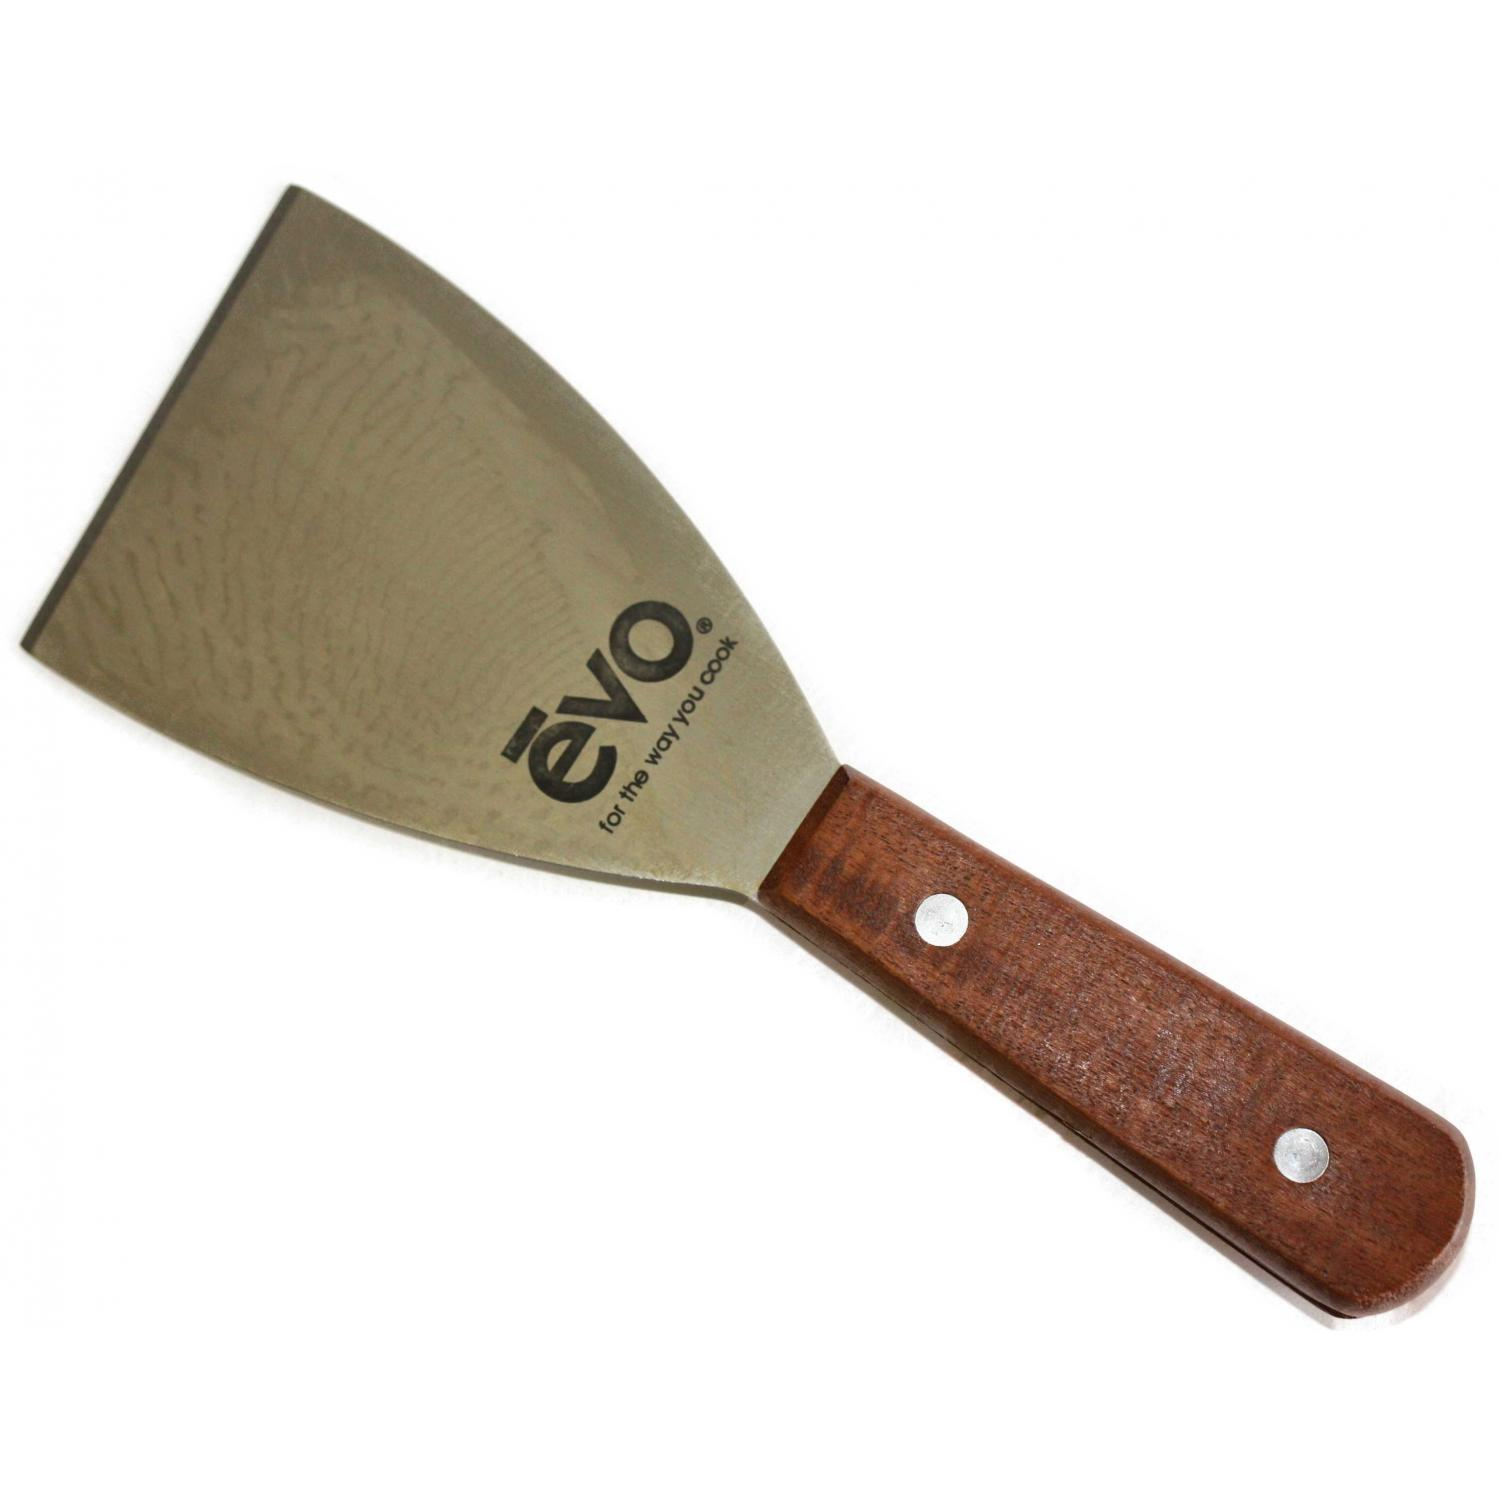
\includegraphics[scale=0.04]{img/icons/scraper.jpg}
\end{minipage}

\end{frame}



\subsection{Legality of Web Scraping}
\begin{frame}
    \frametitle{Legality of Web Scraping}

\begin{itemize}
    \item It is public / Google does it
    \begin{itemize}
    \item Search engines add value
    \item Log in systems, paywalls, ...?
    \end{itemize}
\end{itemize}

\begin{itemize}
    \item Highly context specific
    \begin{itemize}
    \item Commerical v non-commercial
    \item Internal v third party use
    \end{itemize}
\end{itemize}

\begin{itemize}
    \item Technicalities
    \begin{itemize}
    \item Bandwidth usage
    \item Denial-of-service (DoS) attack
    \end{itemize}
\end{itemize}

\end{frame}


\begin{frame}
    \frametitle{European Union}
    \begin{itemize}
        \item \textcolor{iseblue}{Ryanair Ltd v PR Aviation BV (2015)}
        \begin{itemize}
            \item PR Aviation: price comparison of flights
            \item Copyright and database right infringement?
            \item ToS prohibited data extraction for commercial purposes
        \end{itemize}
            \end{itemize}
        \begin{itemize}
        \item Decision by Court of Justice of the European Union
        \begin{itemize}
            \item No infringement of intellectual property, no creative input
            \item ToS still apply, liability in terms of breach of contract
        \end{itemize}
    \end{itemize}
    \vspace{5pt}
        \begin{itemize}
        \item In contrast \textcolor{iseblue}{NLA v Meltwater (2013)}
        \begin{itemize}
            \item Scraping of news headlines and links to articles
            \item Intellectual property is infringed because of creative input
        \end{itemize}
    \end{itemize}
\end{frame}

\begin{frame}
    \frametitle{United States}
\color{isegreen}{\textbf{Pro}} \\
\begin{itemize}
    \item Web data is public, should be accessible
    \item Unfair market power of Facebook, Google, LinkedIn, ...
    \item First Amendment protects information gathering
\end{itemize}
\vspace{8pt}
\color{isered}{\textbf{Contra}} \\
\begin{itemize}
    \item Copyright infringement
    \item Breach of contract
    \item Violation of the Computer Fraud and Abuse Act (CFAA), 1986
    \item Trespass to chattels
\end{itemize}
\end{frame}

\begin{frame}
    \frametitle{LinkedIn v hiQ and vice versa}
{
\center
\textit{
\large
If you exclude someone from sites like LinkedIn, Facebook and Twitter, you are excluding them from the modern version of the town square. }
} \\
\vspace{-10pt}
\begin{flushright}
Laurence Tribe, Harvard law professor
\end{flushright}
\vspace{10pt}
\begin{itemize}
    \item hiQ predicts who is when quitting their job
    \item LinkedIn: CFAA violation, hiQ: blocked
    \item LinkedIn ordered to give access to public profiles
\end{itemize}
\end{frame}

\begin{frame}
    \frametitle{Academia is save, right?}
    \setlength\tabcolsep{1.pt}
      \begin{tabular}{cl}
      \setlength\tabcolsep{1.5pt}
         \begin{tabular}{c}
           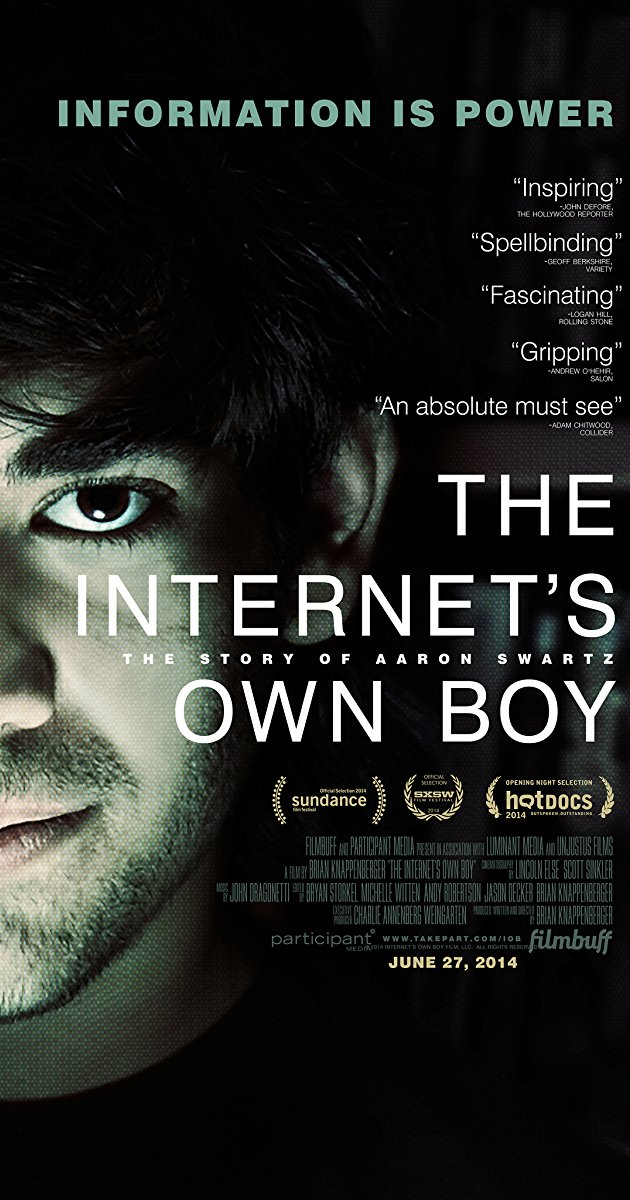
\includegraphics[scale=0.15]{img/figures/aaron_swartz.jpg}
           \end{tabular}
           & \begin{tabular}{l}
            \small
             \parbox{0.7\linewidth}{%  change the parbox width as appropiate
             \textbf{Aaron Swartz} 
             \begin{itemize}
    \item Harvard research fellow
    \item Automatic download of JSTOR articles
    \item Laptop in restricted closet at MIT
    \item No civil law suit by MIT and JSTOR
    \item Federal charges: wire fraud, CFAA violations
    \item Possible penalty of \$1 million and 35 years in prison
\end{itemize}
\vspace{10pt}
Unclear outcome, suicide on January 11, 2013
    }
         \end{tabular}  \\
\end{tabular}   
\end{frame}

\begin{frame}[plain]
\vspace{-82pt}
\hspace*{-32pt}
    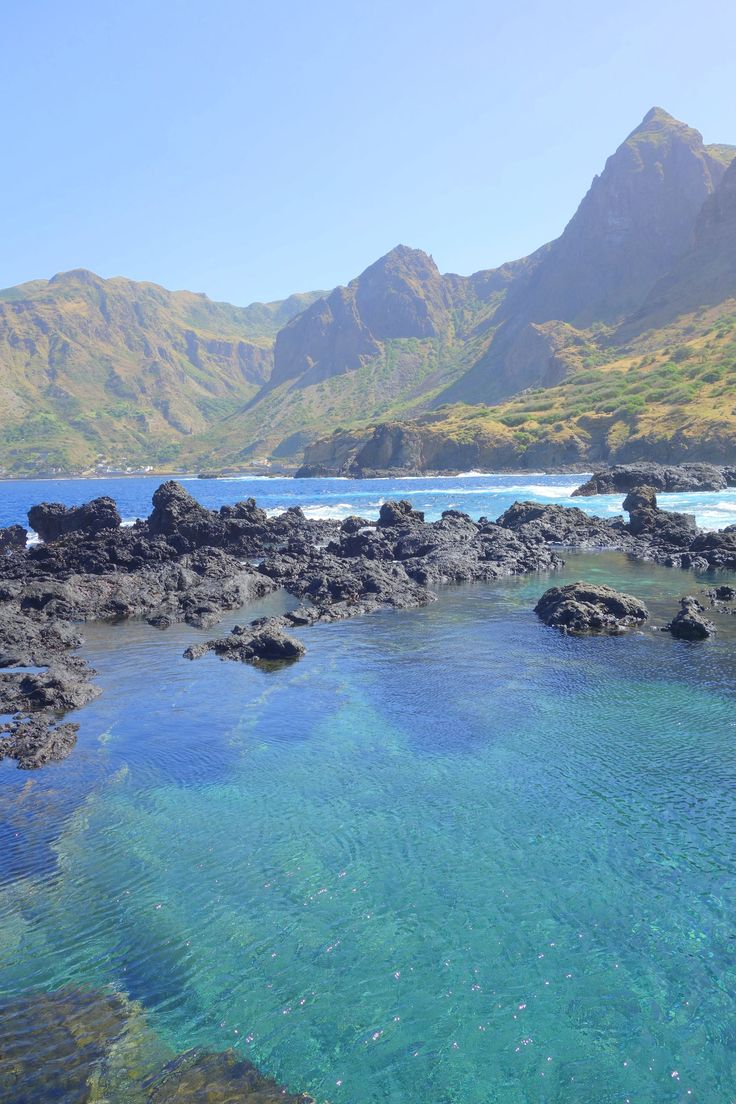
\includegraphics[height=\paperheight]{img/figures/cap_verde}
\vspace{-9cm}
\hspace*{5.5cm} \textcolor{isered}{\Large \textbf{Bright Side}}\\[0.6\baselineskip]
\hspace*{5.5cm} Cap Verde is beautiful and \\[0.2\baselineskip]
\hspace*{5.5cm} does not extradite
\vfill
\end{frame}


\begin{frame}
\frametitle{Ethical Scraping for Academia}
\label{manners}
\begin{itemize}
    \item Technical
    \begin{itemize}
    \item Use API if provided
    \item Appear as a bot, not as a human
    \item Provide user agent string with contact data
    \item Decreased rate of requests
    \item Check robots.txt $\,$ \hyperlink{robots}{\beamerbutton{Google's robots.txt}}
    \end{itemize}
    \end{itemize}
    \vspace{5pt}
    \begin{itemize}
    \item Usage
    \begin{itemize}
    \item Strictly non-commercial
    \item Restrict further access to academia
    \end{itemize}
\end{itemize}
    \vspace{5pt}
    \begin{itemize}
    \item Ask for permission, not for forgiveness!
    \end{itemize}
\end{frame}


\begin{frame}
    \frametitle{Scraping How To}
\hspace*{-0.5cm}
\vspace{-8pt}

\includegraphics[scale=0.15]{img/logos/python}
        \begin{itemize}
        \item Complete framework: Scrapy
        \item Fast and easy: Beautiful Soup
        \item Low level: lxml
    \end{itemize}

\vspace{15pt}
\hspace*{0.1cm}

\includegraphics[scale=0.03]{img/logos/r}
\vspace{-2pt}
    \begin{itemize}
        \item Complete framework: RCrawler
        \item Fast and easy: rvest
        \item Low level: XML
    \end{itemize}

\end{frame}

\begin{frame}
    \frametitle{
\includegraphics[scale=0.2]{img/logos/beeradvocate}}
    \vspace{-15pt}
\begin{itemize}
    \item Largest beer rating community
    \item Founded in 1996, print magazine since 2006
    \item Mostly ``exotic'' and craft beer
\end{itemize}
\begin{itemize}
    \item Still independent
    \begin{itemize}
        \item Anheuser-Busch InBev acquires beer related websites
        \item Examples: RateBeer, The Beer Necessities, ...
    \end{itemize}
    \end{itemize}
        \begin{itemize}
    \item Breweries in the US
    \begin{itemize}
        \item Less than 100 in 1980s, more than 5,000 in 2016
        \item Craft beer boom 
    \end{itemize}
\end{itemize}
\end{frame}

\begin{frame}
    \frametitle{Individual Review}
    \vspace{-25pt}
    \begin{figure}[htb]
        \begin{center}
            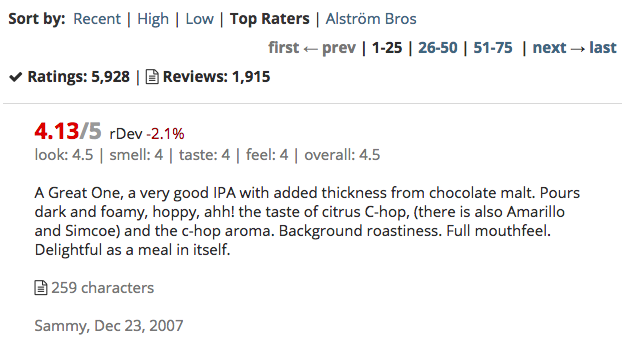
\includegraphics[scale=0.5]{img/figures/rating}
        \end{center}

\end{figure}
\vspace{-20pt}
\begin{flushright}
\textcolor{iseblue}{\href{https://www.beeradvocate.com/beer/profile/147/38470/?view=beer&sort=topr&start=0}{Source}}
\end{flushright}
\end{frame}

\begin{frame}
    \frametitle{xPath Inspector}
    \vspace{-25pt}
    \begin{figure}[htb]
        \begin{center}
            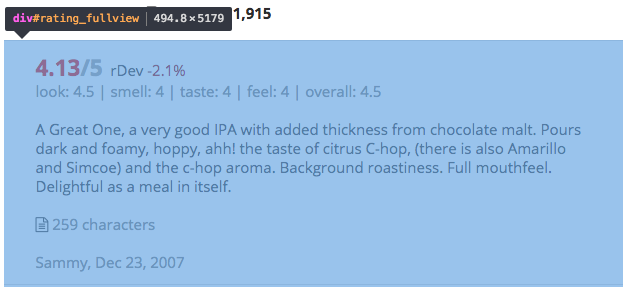
\includegraphics[scale=0.5]{img/figures/xpath}
        \end{center}

\end{figure}
\vspace{-20pt}
%\verb | //*[@id="rating_fullview_content_2"]|

\end{frame}


\frame[plain]{
    \center \LARGE \bf
    \color{isegreen} Example: \href{http://localhost:8888/notebooks/live_examples/scraper.ipynb}{Scraper}
}